%%%%%%%%%%%%%%%%%%%%%%%%%%%%%%%%%%%%%%%%%%%%%%%%%%%%%%%%%%%%%%%%%%%%%%
%
%  Epigenetic Robotics 2006
%
%  We are using SAB format.
%  Choose  'a4' for your draft.
%  (Note that the final proceedings will be using A4 paper.)

\documentclass[a4]{epirob}

%  usepackage goes here.

\usepackage{graphicx}

%%%%%%%%
%
%  title/author/affiliation go here.
%  Note: we slightly changed the use of author/affilication.
\title{A sensitive approach to grasping}

%
%  For one-to-one authur/affil correspondence

%\author{Lorenzo Natale\\
%   \rm  Massachusetts Institute of Technology\\
%   \rm  Computer Science and Artificial Intelligence Laboratory\\
%   \rm  32 Vassar St. Room 32-380\\
%   \rm  Cambridge, MA 02139 US\\
%   \rm  lorenzo@csail.mit.edu
%  \and
%        Eduardo Torres-Jara\\
%   \rm  Massachusetts Institute of Technology\\
%   \rm  Computer Science and Artificial Intelligence Laboratory\\
%   \rm  32 Vassar St. Room 32-380\\
%   \rm  Cambridge, MA 02139 US\\
%   \rm  etorresj@csail.mit.edu}
%
%\affiliation{} % not used in one-to-one mode

%
%  For N-to-M author/affil correspondence
%
  \author{Lorenzo Natale$^{*}$$^{\dag}$\\
          \rm  lorenzo@csail.mit.edu
        \and
          Eduardo Torres-Jara$^{*}$\\
          \rm  etorresj@csail.mit.edu}
  \affiliation{$^{*}$Massachusetts Institute Technology\\
    \rm  Computer Science and\\
    \rm Artificial Intelligence Laboratory\\
    %\rm  CSAIL\\
    %\rm  32 Vassar St. Room 32-380\\
    \rm  Cambridge, MA 02139 US\\
             \and
              $^{\dag}$\rm  University of Genoa\\
   \rm  LIRA-Lab, DIST\\
   \rm  Viale F. Causa 13\\
   \rm  16145 Genoa, Italy
   }

%%%%%%%%
%
%  Local setting (if any) goes here.

%  Now, let us begin.

\begin{document}

\maketitle

\begin{abstract}

The importance of interacting with the environment has been stated
by the embodied intelligence field and for development. There are
many ways to interact with environment but the physical contact is
he most common in biological agents. That is why animals are
provided by limbs. pwas, etc. All of them covered by a higly
inervated skin that allows them to get intimate informatino about
their phyisical enviroment. This interaction helps them to develop
the skills needed for their survival and is done in a safe way.
Interaction with the enviroment is key for the robtos, with outhe
posibility of the interactions very little can be done.  In this
paper we show how a robot can explore its enviromante, feel
objects and grasp them only by using tactile and force feedback
information. The interaction is safe and useful. In other words,
the robot can come in actual physical contact with its
environment. Many efforts in robotics has been done about learning
from the environment by interacting with it. However, the
interaction has been very rough. This works will present an
alternative to fill this grasp. ALthough this is not the ultimate
goal.


%Humans use a set of exploratory procedures to examine object
%properties through grasping and touch. Our goal is to exploit
%similar methods with a humanoid robot to enable developmental
%learning about manipulation. We use a compliant robot hand to find
%objects with very rough estimation about their location, and then
%tap grab them. This behavior lets the robot collect samples of the
%grasping of that object.
%
%An important property of embodied agents is their ability to
%interact with the environment in which they operate. This is
%considered of fundamental importance for the emergence of
%intelligent behavior. Recent work in robotics has shown how simple
%actions (like poking and prodding) can facilitate perception and
%learning1. Grasping is particularly appealing in this context
%because provides direct access to physical properties of objects
%(like shape, volume and weight) that are difficult to perceive
%otherwise. Unfortunately this aspect has rarely been investigated,
%with a few exceptions2,3. In part this is because current robots
%have very limited perceptual capabilities. In particular, tactile
%sensing is often inadequate or inexistent. For this reason most of
%the research on manipulation has focused on vision and has left
%haptic sensing overlooked. This paper pushes the idea that
%sensitive haptic feedback dramatically simplifies manipulation and
%improves the ability of robots to successfully interact with
%unknown objects. In this paper we report a series of experiments
%recently performed on Obrero. The robot exploits its sensing
%capabilities to grasp a number of objects individually placed on a
%table. No prior information about the objects is available to the
%robot. Vision is used at the beginning of the task to direct the
%attention of the robot and to give a rough estimation of the
%position of the object. Tactile feedback allows the robot to
%refine this initial estimation during the task. The robot reaches
%for the object and explores with the hand the area around it.
%During exploration the robot exploits tactile feedback to find the
%actual position of the object and grasp it. The mechanical
%compliance of the robot and the control facilitate the exploration
%by allowing a smooth and safe interaction with the object. In
%figure 2, we observe a sequence of the robot grasping one of the
%objects. Preliminary analysis of the data collected in these
%experiments shows that the haptic feedback originated by the
%interaction between the objects and the robot carries information
%useful for learning.


\end{abstract}

\section{Introduction}
Put here the introduction.
%

\section{Haptic feedback, perception and action}
\label{sec:background}

In adults, several studies have revealed the importance of
somatosensory input (force and touch). For example Johansson and Westling
\cite{Johansson90Tactile} have studied in detail what feedback
is provided by the skin during object lifting tasks and how it is
used to control the movements of the fingers. The results of these
experiments proved the importance of somatosensory feedback: they
showed that human subjects had difficulties avoiding object slipping when
they had their fingertips anesthetized, even with full vision
\cite{johansson91how}. 

Haptic feedback has an important role for
object perception as well. Lederman and Klatzky \cite{klatzky87Hand}
identified and described a set of motor strategies --- or 
\emph{exploratory procedures} --- used by humans to determine 
properties of objects such as shape, texture, weight or volume.

Little is known concerning how infants use 
tactile sensing for manipulation \cite{streri93Seeing}.
%Tactile sensing in neonates is very poorly known
%in contrast to the visual mechanism\cite{streri93Seeing}.
%However, tactile sensing provides information to children since
%his time in the wound. 
In some circumstances children exploit tactile feedback to learn
about objects \cite{streri86Habituation}. Streri and P\^{e}cheux
measured the habituation time of newborns (2 months and 5 months
old) during tactile exploration of objects placed in their hands.
In this experiment children spent more time exploring novel rather
than familiar objects, even when they did not make visual contact
with the hand. %This experiment was repeated with visual feedback
%showing the same behavior.

Motor abilities of children are quite
limited during the first months of development. This does not
prevent infants from using their hand to engage interaction
with the world. The importance of motor activity for perceptual 
development has been emphasized in developmental psychology 
\cite{hofsten04motor,gibson88explore}. Researchers agree on
the fact that motor development determines the timing of
perceptual development. In other words the ability of infants 
to explore the environment would determine their capacity to 
perceive certain properties. 
Accordingly, perception of object features like temperature, 
size and hardness is likely to occur relatively early in development, 
whereas properties requiring more dexterous actions like texture or 
three dimensional shape would emerge only later on (see \cite{bushnell93motor} 
for a review).
%% Later on in development the integration between visual and tactile
%% modalities during reaching tasks has been found. Tactile
%% information is, for example, used to confirm visual stimulus as
%% described in \cite{bower70Coordination}. In this experiment an
%% image of an object was projected used polarized lenses so that
%% children wearing ``stereo'' glasses perceived a 3D object.
%% Children of different ages were tested in two conditions: when the
%% object was actually present and when it was not. Older children (5
%% to 6 months-old) showed surprise when the did not feel the contact
%% when expected, whereas the younger ones closed their hand to grasp
%% the object \textbf{[X and  did not show any surprise. * This is
%% not true. Both showed surprise. Also, I am not sure if its later
%% because the experiment was done with children from 6 days to 6
%% months. And we do not know if they were tested in the both
%% conditions. X]}
%

\section{The robot Obrero}
\label{sec:platform}


\begin{figure}[tbp]
\centerline{
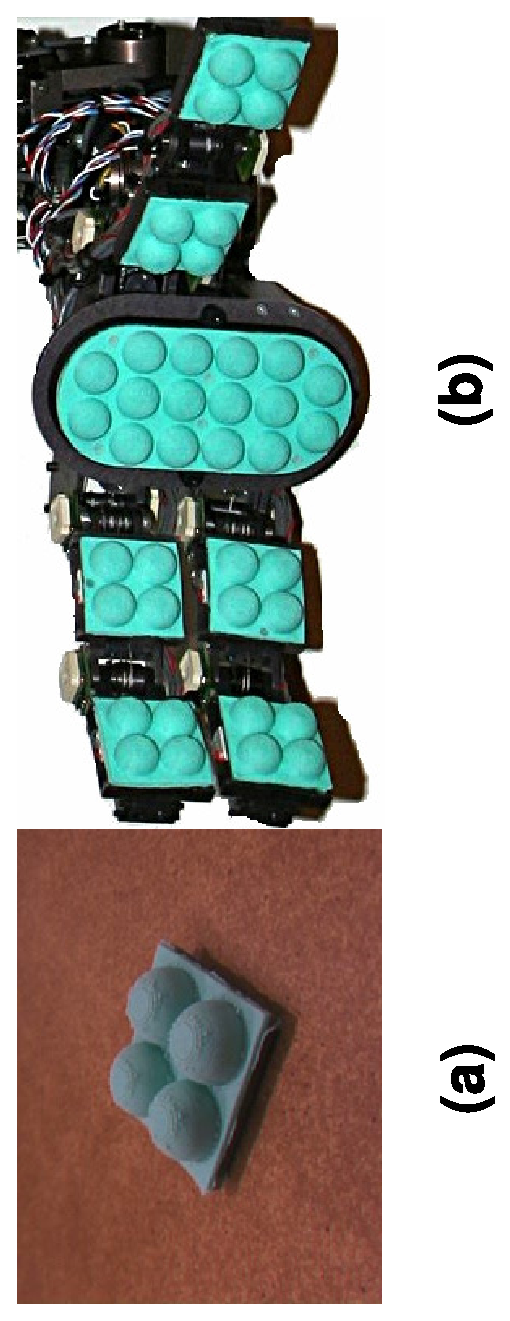
\includegraphics[width=1.0in, angle=270 ]{./figures/Tactiles.eps}
} \caption{Tactile Sensors. (a) Group of four tactile sensor. A
total of 16 sensors are read to determine the deformation of the
four tactile sensors. (b) Tactile sensors mounted on Obrero's
hand.} \label{fig:TactileSensors}
\end{figure}

Obrero \cite{obrero} consists of a hand, an arm and a head
(Figure~\ref{fig:RobotObrero}). Obrero was designed to approach
manipulation as a task manly guided by tactile and force feedback.
We use the robot's limb as a sensing/exploring device as opposed
to a pure acting device. This is a convenient approach to operate
in unstructured environments, on unmodeled objects. Obrero's limb
is sensor-rich and safe, it is designed to reduce the risk of
damages upon contact with objects. The head consists of a
commercial camcorder (SONY DCR-HC20) that can move along the pan
and tilt directions. The arm has 6 Degrees of Freedom (DOF)
distributed in this way: three in the shoulder, one at the level of the
elbow and two in the wrist. The arm mounts Series Elastic Actuators
\cite{williamson95series} which provide low-impedance and force
feedback at each joints (\cite{AaronArm}). Position feedback is
provided by analog encoders (potentiometers).

The hand consists of a palm, a thumb, a middle and an
index finger. Each one of the fingers has two links that can be
opened and closed. The thumb and the middle finger can also
rotate. These rotations allow the the thumb to oppose to either
the index or the middle fingers.

%By rotating the thumb it can be opposed to the index
%finger and by rotating the thumb and the middle, they can oppose
%to each other.

The total number of degrees of freedom in the hand is 8. The hand
is underactuated, only 5 motors are connected to the fingers. Three motors control
the opening and closing of the fingers. The remaining two motors actuate
the rotation of the thumb and middle finger. The phalanges in each fingers
are mechanicaly coupled and actuated by a common motor. The link between
the two joints is realized by means of Series
Elastic Actuators, to allow independent motion
whenever one of the phalanges blocks (for example as a result of contact
with an object). This elastic coupling allows the hand to automatically
adapt to the object it grasps. All joints in the hand are equipped with an
optimized version of the Series Elastic Actuators \cite{actuator} which provide
force feedback and reduce the mechanical impedence of the fingers. Finally
position feedback is obtained through analog encoders mounted in all joints.

%However, they can decouple thanks to the SEA's in each
%joint. All the joints of the hand are controlled using an
%optimized design for a series elastic actuator \cite{actuator}.
%There are a total of 8 SEA's int the hand. Series elastic
%actuators\cite{williamson95series} reduce their mechanical
%impedance and provide force sensing.

The tactile sensors mounted on the robot were designed for robotic tasks.
Their design was inspired by the dome-like shape of the ridges that have been
observed in the human skin, where the innervations at the base of the ridges
detect the deformation of the skin.

Inspired by this mechanism we realized a tactile sensor made of
silicon rubber and with a dome-like shape (see
figure\ref{fig:TactileSensors}a). At the tip of the dome, in the
internal part, we mounted a small magnet, whose position is
measured by four hall-effect sensors placed at the base. The
hall-effect sensors in this way measure the deformation of the
dome by sensing the position of the magnet at the tip. The sensors
are very sensitive and have been tested to detect up to the
minimum normal force of 10g.

The shape the sensors favors contact with the environment from any direction,
as opposed to most of the tactile sensors which are flat.
This high deformability and the properties of the silicon rubber allow the
sensors to conform to the objects, thus increasing friction and improving
contact detection.

In the particular implementation used in this paper, we used the
''magnetic'' version of the tactile sensors, however, a optical
version has been also tested. An analysis and description of the
design of these sensors can be found in \cite{etorresjSoft}.
Groups of tactile sensors were placed in parts of the hand. Two
groups of four were placed on each finger (a group in each of the
two phalanges) and 16 on the palm. A detail of the palm and
fingers can be observed in figure\ref{fig:TactileSensors}b . Each
one of these tactile sensors uses 4 sensors to determine the
contact forces. That means that overall the tactile feedback
consist of 160 sensors. At the base of the palm, where for
practical reasons, we were not able to mount these tactile
sensors, we placed a smaller infrared proximity sensor. To
summarize, the hand has 5 motors, 8 DOF, 8 force sensors, 10
position sensors, 160 tactile sensors and a infrared proximity
sensor.

\section{Overall developmental approach}
 \label{sec:approach}
[Should we keep this?]

 We wish to give our robots many ways to learn about
objects through action (Fitzpatrick et al., 2003). This
contributes to perceptual development, where the robot's
experience of the world is filtered by prior experience. This
process can be broken down into four steps:

\begin{itemize}

\item Identification of an opportunity to reliably extract some
object features.

\item Exploitation of that opportunity to extract those features.

\item Use careful generalization to transform the robot's
perception of its environment.

\item Transformation of the robot's activity, enabled by its
extended perceptual abilities.

\end{itemize}

In previous work, we have demonstrated this process. In (Arsenio
et al., 2003), we showed that poking an object gives us the
opportunity to reliably extract visual features of its appearance.
By carefully choosing features that generalize, the robot's
perception of its environment is transformed, and new activities
are enabled (Fitzpatrick, 2003b). Other opportunities we have
explored include the use of grasping (Natale et al., 2005) and the
integration of multi-modal cues across sound, vision, and
proprioception (Fitzpatrick et al., 2005, Arsenio and Fitzpatrick,
2005). Having established this process, we are now seeking to
broaden the range of opportunities that can be identified and
exploited Figure 3: The component elements of the robot's
behavior. The modules Arm control, Arm sensing, Hand control and
Hand sensing represent the connection with the hardware of the
robot. (steps 1 and 2 above). In the current work, we identify
(and in fact create) an opportunity to reliably extract examples
of contact sounds involving an object (by tapping that object). We
build the appropriate robot behavior and data collection
infrastructure to gather those features.





\section{Controlling the body}
\label{sec:controlling}
%
In this section we describe a few perceptual and motor competencies required
for the robot to be able to control the body in a meaningful and safe way:
this includes a simple attention system to spot the objects to be grasped
and the ability to control the body to reach out for them. A the end of the
section we describe how the these capabilities are integrated in the grasping
behavior.
%
\subsection{Attention System}
Motion is a simple yet powerful cue to select points of interest
in the visual scene; for an active camera system this is still
true assuming we can estimate the motion of the background and
account for it. In this paper we use the algorithm proposed by
\cite{kemp-thesis}, which uses a 2D affine model to robustly
estimate the image motion resulting from the background. In short
the algorithm measures the motion of each pixel with a block
matching procedure, and performs a least square fitting of the
global affine model. Using the affine model the algorithm performs
a prediction of the motion of each edge, and marks as foreground
those edges that poorly match this prediction. Under the
assumption that the majority of the image motion relate to the
background, these edges can be used to build a saliency map to
direct the attention of the robot.
%
\subsection{Eye-hand coordination}
Given the topic of our research, we decided to focus on explorative
actions rather than precise, goal directed, actions towards the target objects.
This was also motivated by the fact that the monocular visual system of Obrero
makes depth estimation very difficult. This situation is actually quite common
in robotics, as depth estimation in real time is a challenging problem even with
stereo vision.
On the other hand, however, we cannot hope to program the robot to perform
a blind exploration of the entire workspace. A possible solution is to
constran the exploration to the area of the workspace where the object is
detected visually. Since the 3D location of the object is not available reaching
is performed in 2D; the exploration procedure allows the robot to find the actual
position of the object. The motor skills required for reaching and performing
the exploration can be learnt starting from the visual abilities
to localize the hand and compute the orientation of the arm.

\subsection{Hand Localization}
A visual module detects the hand and computes the orientation of
the arm in the image. The initial step of the hand detector
consists in running a high frequency filter. All points whose
frequency is below a certain threshold (fixed a priori) are
discarded. A blob detector is run on the resulting image and the
biggest blob is selected as the arm. The orientation of the arm is
computed as the orientation of the line passing through the
top-most and bottom-most pixels of the arm area. Next, specific
features (the small circular black and white potentiometers on the
fingers) are searched on the arm area. The hand is identified if
more than two of these features are found. The detection just
described proved reliable enough for our purposes and was used as
a short-cut in place of other, more general, methods
\cite{metta03early,natale05from}.

The visual feedback of the hand could be used for closed-loop control.
However closed-loop control is not always suitable. This happens for example
in presence of occlusions or when the hand is not within the visual field.

Open-loop control is an alternative solution. A possible open-loop
control consists of a mapping between the fixation point of the
head and the arm end-point \cite{metta00Babybot}. The advantage of
this approach is that the mapping can be easily learnt if the
robot can fixate the hand. Another approach is to use the hand
localization to learn a direct mapping between the arm
proprioception (encoder feedback) and the position of the arm in
the visual space \cite{natale05from}. The direct (forward) mapping
can be inverted locally to control the arm to reach for a visually
identified target. The solution we adopt here is similar: in a
discovery phase the robot tracks the hand as the arm moves to
randomly explore the workspace. This behavior allows the robot to
acquires the samples:
%
\begin{center}
\begin{math}
  \left(\begin{array}{ccccc}
    x & y & \alpha &q_{head} &q_{arm} \end{array}\right)_{0,1\dots,k}
\end{math}
\end{center}
%
where $x$ and $y$ are the coordinates of the hand in the image,
$\alpha$ is the orientation of the arm, $q_{head}$ and $q_{arm}$ are
the position of the head and arm respectively. Given $q_{head}$ it is
possible to convert $x$ and $y$ into an egocentric reference frame:
%
\begin{equation}
  \left[
  \begin{array}{ccc}
    \theta & \phi
    \end{array}\right]^T
  = f_{head}^{-1}
  \left(\left[\begin{array}{ccc}
    x &
    y &
    q_{head}
    \end{array}\right]^T \right)
\label{eq-head-inverse}
\end{equation}
%
$\theta$ and $\phi$ represents the polar coordinates of the hand in the
reference frame centered at the base of the robot. Basically
$f_{head}^{-1}$ includes knowledge of the inverse kinematics of the
head and the parameters of the camera. The opposite transformation maps
polar coordinates into the image plane:
\begin{equation}
  \left[\begin{array}{cc}
    x & y
    \end{array}\right]^T
  = f_{head}
  \left(\left[\begin{array}{ccc}
    \theta &
    \phi &
    q_{head}
    \end{array} \right]^T\right)
\label{eq-head-direct}
\end{equation}

Given these two transformations a neural network can be trained to
learn the following mapping:
%
\begin{equation}
  \left[\begin{array}{ccc}
    \theta & \phi & \alpha
    \end{array}\right]^T=
  = f \left(q_{arm}\right)
\label{eq-arm-direct}
\end{equation}
%
which links the arm posture $q_{arm}$ to the polar coordinates of
the hand $\left[\theta, \phi\right]^T$ and the orientation of the
arm $\alpha$. To learn this mapping we used a neural network
suitable for online learning \cite{schaal98Constructive}.

This mapping allows computing the polar coordinates of the hand
with respect of the robot from the encoders of the arm. Whenever
required Equation~\ref{eq-head-direct} maps the polar coordinates
back onto the image plane.

\subsection{Reaching}
\label{sec:reaching}
%
Suppose we want to move the arm towards a
location of the workspace identified visually. Let
$\left[\begin{array}{c c} x_t & y_t\end{array}\right]^T$ be such
position. Knowing $q_{head}$ from equation \ref{eq-head-inverse}
we can convert the target position into the body centered
reference frame $\left[\begin{array}{c c} \theta_t  &
\phi_t\end{array}\right]^T$. The reaching problem can now be stated
as a the minimization of the following cost function:
%
\begin{equation}
  \displaystyle\min_{q_{arm}}\left(C\right)=\displaystyle\min_{q_{arm}}\left(
  \left[
  \begin{array}{cc}
    \theta_t & \phi_t 
    \end{array}\right]^T
  -f \left(q_{arm}\right)
  \right)^2
\label{eq-reaching1}
\end{equation}
%
Assuming a stationary target the minimum of equation \ref{eq-reaching1}
can be found by gradient descent. The gradient of $C$ is proportional
to the Jacobian transposed of the manipulator, that is:
%
\begin{equation}
  \nabla C=-2\nabla f\left(q_{arm}\right)=-2J^T\left(q_{arm}\right)
\label{eq-gradient}
\end{equation}
%
$\nabla f\left(q_{arm}\right)$ can be approximated by partial
 differentiation of equation \ref{eq-arm-direct}. The
differentiation can be numerical or analytical (the output of the
network can be easily differentiated because the basis functions
used in the neural network are gaussians with known parameters).

To summarize we have described a method to compute the arm
commands required to reach for a visual target. The method employs
the forwards kinematics of the arm. The direct kinematics is
learnt by the robot as described in the previous section. The
reaching problem is solved iteratively by using an approximation
of the arm Jacobian. The latter is obtained by differentiating the
basis functions of the neural network approximating the direct
kinematics. This procedure is carried out online without using the
real visual feedback of the hand.

In the robot visual information (and hence the mapping of equation~\ref{eq-arm-direct})
is two-dimensional and does not carry any information
about distance. The solution found by descending the gradient of the
direct kinematics takes care of minimizing the distance between the target
and the hand \emph{on the image plane}, and as such, is not concerned
with the third dimension $R$ (the distance between the hand and the image
plane, along the optical axis).
In practice however the components of the gradient along $R$ are small
compared to the others. The value of $R$ at the end of the reaching movement
depends on the initial position of the arm; we chose this value so to keep
the hand above the table.
%
\begin{figure}[tb]
  \centerline{
    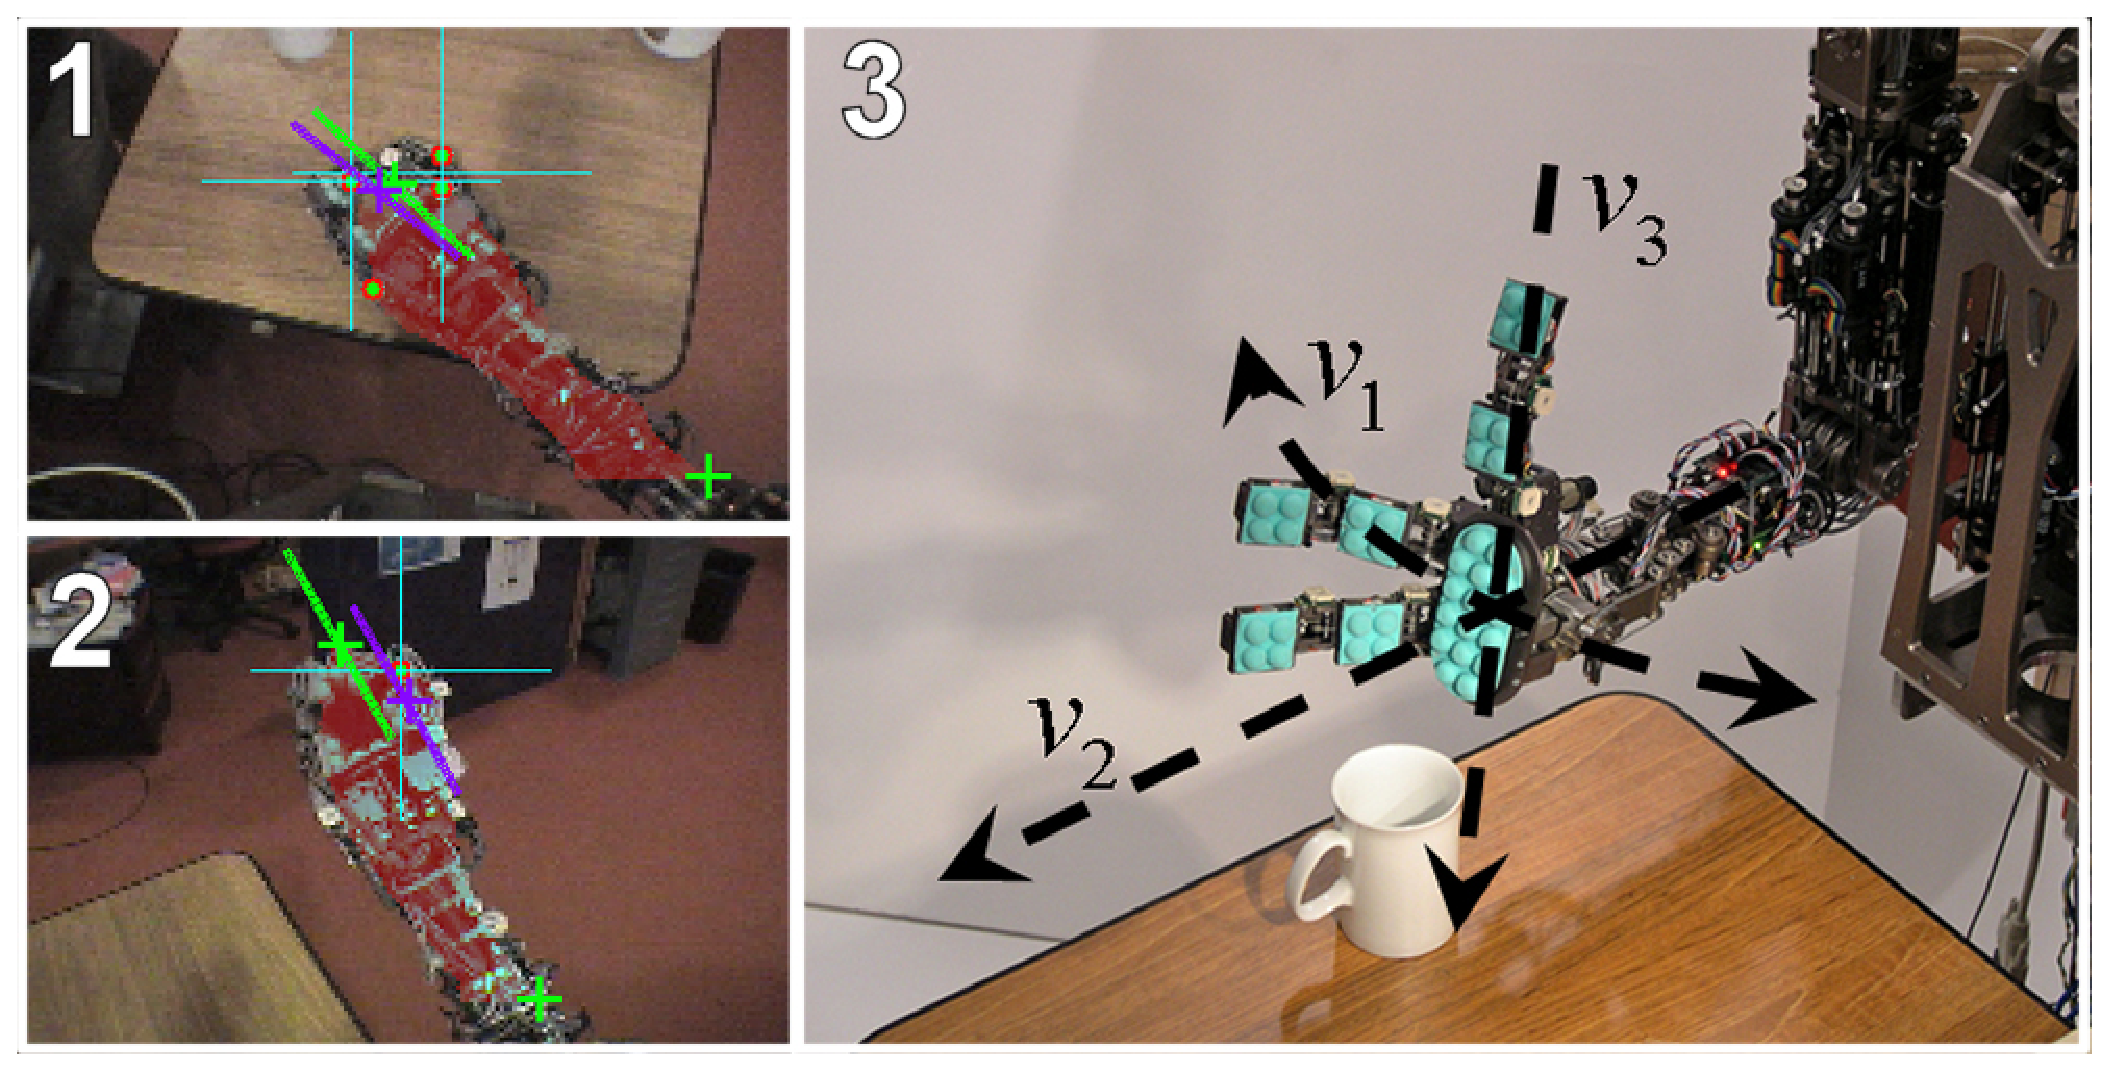
\includegraphics[width=\columnwidth, angle=0 ]{./figures/expl-directions.eps}
  }\caption{Left, frames 1 and 2: hand localization and arm
    orientation. Right, frame 3: exploration primitives. Primitives $v_1$
and $v_3$ are perpendicular and parallel to the arm orientation.
$v_2$ is along the null space of the arm Jacobian. See
section~\ref{sec:controlling} for
 more details.}
\label{fig:expl-directions}
\end{figure}
%
\subsection{Exploration}
Starting from the direct mapping of the hand position and arm orientation we
can identify a set of explorative primitives, that is a set of vectors in
joint space that allows the robot to explore the arm workspace. We chose three
vectors $v_1$, $v_2$ and $v_3$, as follows:

$v_1$: moves the hand along the
direction perpendicular to the arm. It is computed by planning a 
reaching movement towards a point a few pixels away from the hand along the
line perpendicular to the orientation of the arm.

$v_2$: moves the hand along the
direction of the arm. It is computed by planning a 
reaching movement towards a point a few pixels away from the hand along the 
arm.

$v_3\in \ker \left(J\left(q_{arm}\right)\right)$
%
$v_3$ lays in the null space of the arm Jacobian; in our case the
null space of the Jacobian consists of those vector that do not affect
either the projection of the hand onto the visual plane or the orientation
of the arm. These vectors produce a movement of the hand along the optical
axis of the camera, or, in other word, along $R$.
$v_1$, $v_2$ and $v_3$ are depicted schematically on the left side of
Figure~\ref{fig:expl-directions}.
%
\subsection{A grasping behavior}
In this section we describe the grasping behavior of the robot.
The sequence begins when the experimenter waves an object in front
of the robot. The head tracks the object until it remains
stationary within the workspace of the arm. The robot reaches for
the object; motion is planned visually as described in
section~\ref{sec:reaching}. Reaching is not accurate enough to
guarantee a correct grasp. Since no three dimensional information
is available the arm reaches a region above the object (see
section~\ref{sec:reaching}). At this point the exploration starts;
the robot computes the explorative primitives $v_1$, $v_2$ and
$v_3$. The exploration mainly uses three behaviors: 
%
\begin{itemize}
\item \emph{hovering behavior}, moves the hand back and forth along 
$v_1$ 
%
\item \emph{pushing behavior}, moves the hand
along $v_2$ 
%
\item \emph{depth behavior}, moves the hand ``downwards''
along $v_3$; this behavior moves the hand along the direction of
the optical axis of the camera and adjusts the height of the hand
with respect to the object/table. To avoid crashing the hand into
the table this behavior is inhibited when the infrared proximity
sensor detects an obstacle (usually this happens close to the
table).
%
\end{itemize}
%
The \emph{hovering behavior} and the \emph{depth behavior} are
activated at the beginning of the exploration. The goal of this
initial phase is to adjust the position of the hand until the
index finger touches the object. This allows adjusting the
position of the hand along the directions $v_1$ and $v_3$. During
the exploration the arm stops when the hand detects the object, to
avoid pushing it away or knocking it over; if no contact is
detected, on the other hand, the amplitude of the exploration is
extended (this increases the probability to touch the object in
case the reaching error is large); the exploration terminates when
the contact with the object is detected by any of the tactile
sensors placed on the index finger. At this point the \emph{hovering
behavior} is suspended and the \emph{pushing behavior} activated. The
``pushing'' movement along $v_2$ brings the palm in contact with
the object while the \emph{depth behavior} takes care of
maintaining the correct distance with the table. When the robot
detects contact on the palm the exploration stops and the
\emph{grasping behavior} is activated. The \emph{grasping
behavior} simply closes the fingers to a specific position. The
low impedance of the joints allows the fingers to adapt to the
different objects being grasped.

The grasping behavior proved to be quite reliable. Figure \ref{fig:sequence}
shows an example of the robot grasping a porcelain cup. Repetitive tests
are described in section \ref{sec:results}
\section{Results}
\label{sec:results}

In this section we report the results of the experiments we carried out
to quantify the performance of the reaching movements. Following the proposed strategy, 
in order to reach for the 
target we first need to fixate it, i.e. $\utarget = 0$. Using the available sensor (i.e. vision) the best we can do to precisely reach the target is moving the hand to the fixation point, i.e. $
{\uhand} \longrightarrow 0$. Clearly, the image plane distance $\| \uhand - \utarget \|$ can be used as a rough estimate of the reaching precision, i.e. of the Cartesian distance between the target to be reached and the position of the hand. Specifically, assuming infinite resolution of the camera sensor, if $\| \uhand - \utarget\| = 0$ then the hand has exactly reached the target.

\subsection{Open Loop}
The first attempt to reach the target consists in using the learned forward model 
(\ref{Eq:forward}) and the strategy (\ref{Eq:reaching2})
to choose the arm configuration $\q_{arm}$ which brings the hand to the center 
of the image planes. Clearly, if the forward 
kinematic function (\ref{Eq:forward}) were perfectly represented and if the target were reachable, then we would have 
$\mathbf x_{hand} =  \mathbf x_{target}$, which implies that the target-hand Cartesian distance 
 is zero (see Section \ref{sec:reaching} for details). Therefore, in this ideal case, the open loop 
 strategy already results in $\| \uhand - \utarget \| = 0$. In practice, the model 
 (\ref{Eq:forward}) cannot exactly represent the system's kinematic\footnote{Part of the representational 
 errors are related to the representation of the kinematic function, in this case the
 so called Receptive Field Weighted Regression model. Part are due to the mechanical plays and backlash of the
 mechanical structure.}. Therefore, even tough we can find $\q_{arm}$ such that $\mathbf x_{hand}=
 \hat f_{arm}(\mathbf q_{arm})$ it is not guaranteed that after the movement execution 
 $\| \uhand - \utarget \| = 0$. Figure \ref{Fig:ImagePlaneOpenLoopErrors}
 shows the image plane errors after the execution of the open loop movement. The plot has been obtained
 by fixating a target and performing a series of open loop movements. Each open loop
 movement was different because (\ref{Eq:reaching2}) was solved 
 by choosing a different value $q_{20}$. 


\begin{figure}
  % Requires \usepackage{graphicx}
  \begin{center}
	\begin{tabular}{ccc}
	  \parbox{30mm}{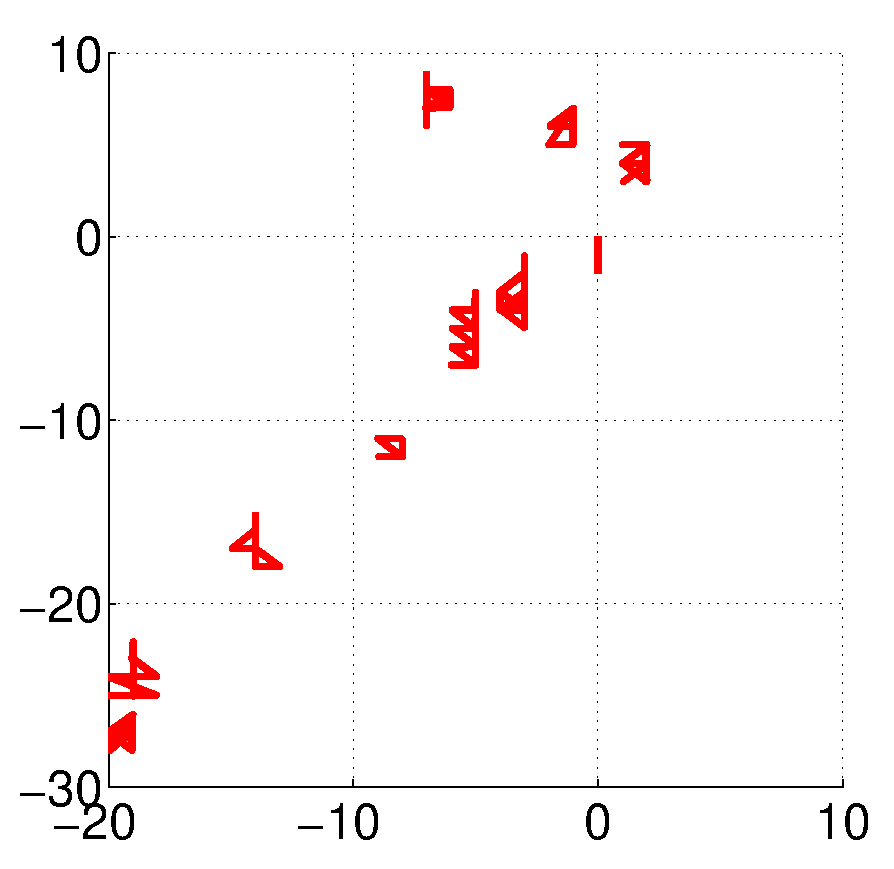
\includegraphics[width=30mm]{Figure/LeftEyeOpenLoop.eps}}  & \hspace{0.1cm} &
	  \parbox{30mm}{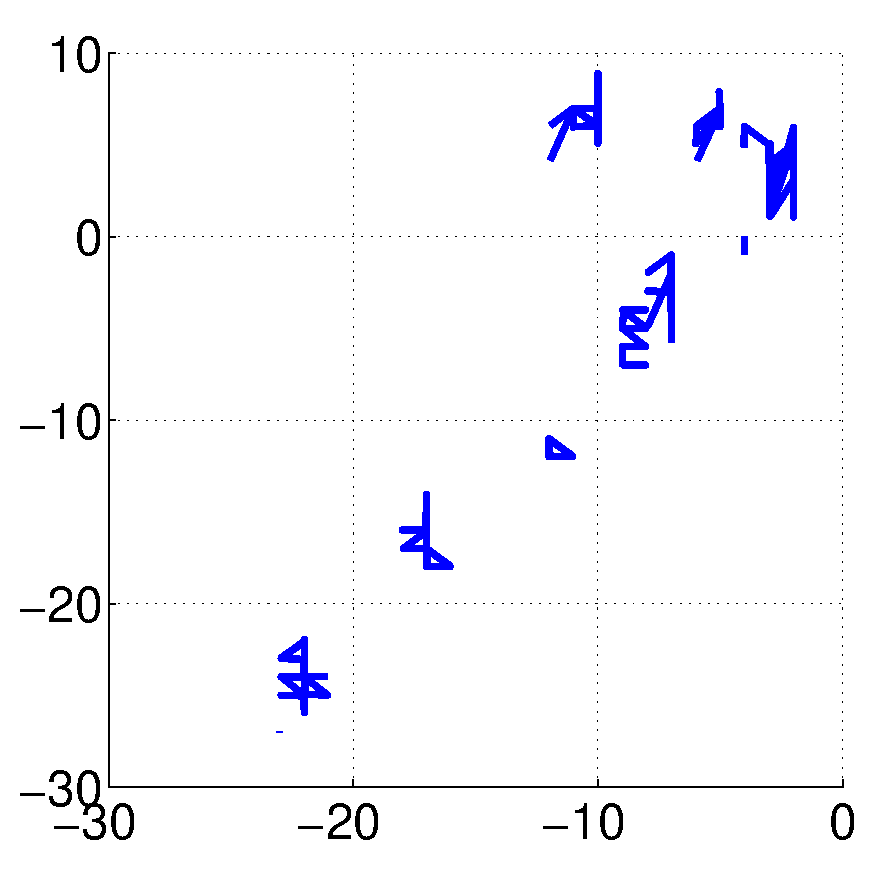
\includegraphics[width=30mm]{Figure/RightEyeOpenLoop.eps}}
	  \\
	  \parbox{30mm}{\centering Left eye } & \hspace{0.1cm} & \parbox{30mm}{\centering Right eye }
	  %	  \end{t\\
	  %	Top view & & Lateral view
  \end{tabular}
\end{center}
\caption{Open loop image plane errors $\uhand$ for different
choices of the redundant variable $q_{20}$. On the horizontal axis 
$u_r$ and $u_l$; vertical axis $v_r$ and $v_l$ (always in pixels).
The hand position in the image plane is represented 
by the small circles.  Each circle corresponds to a different open loop movement, i.e. a different value of $q_{20}$.
}\label{Fig:ImagePlaneOpenLoopErrors}
 \end{figure}

\subsection{Closed Loop}

The residual image plane errors 
due to imperfections in the forward kinematic model can be reduced by a visual closed loop
control strategy (\ref{Eq:ClosedLoopStrategy}), started immediately after the open loop phase. Relatively weak conditions on the learned 
Jacobian \cite{Samson91robot} guarantee the convergence of the image plane errors $\uhand$ to zero, and therefore
the convergence of the hand $\xhand$ on the target $\xtarget$. Figures
\ref{Fig:ImagePlaneClosedLoopErrors}, %\ref{Fig:TimeResponseClosedLoopErrors}, 
\ref{Fig:TimeResponseOpenClosedLoopErrors} and \ref{Fig:TimeResponseOpenClosedLoop}  
show how the hand is actually driven to the 
exact image center in both the image planes. The closed loop controller 
improves the accuracy of the reaching movement, but at the cost of a slower 
execution speed (see Figure \ref{Fig:TimeResponseOpenClosedLoop}); faster
executions couldn't be obtained by increasing the control loop gains, due to
the frame rate (thirty milliseconds) and the delays in the visual processing (hand localization and tracking).
Finally, it is important to notice 
the quasi-linearity of the path followed by the hand 
(see Figure \ref{Fig:ImagePlaneClosedLoopErrors}). This linearity denotes 
a good accuracy of the learned Jacobian.

\begin{figure}[th!]
  % Requires \usepackage{graphicx}
  \begin{center}
	\begin{tabular}{ccc}
	  \parbox{30mm}{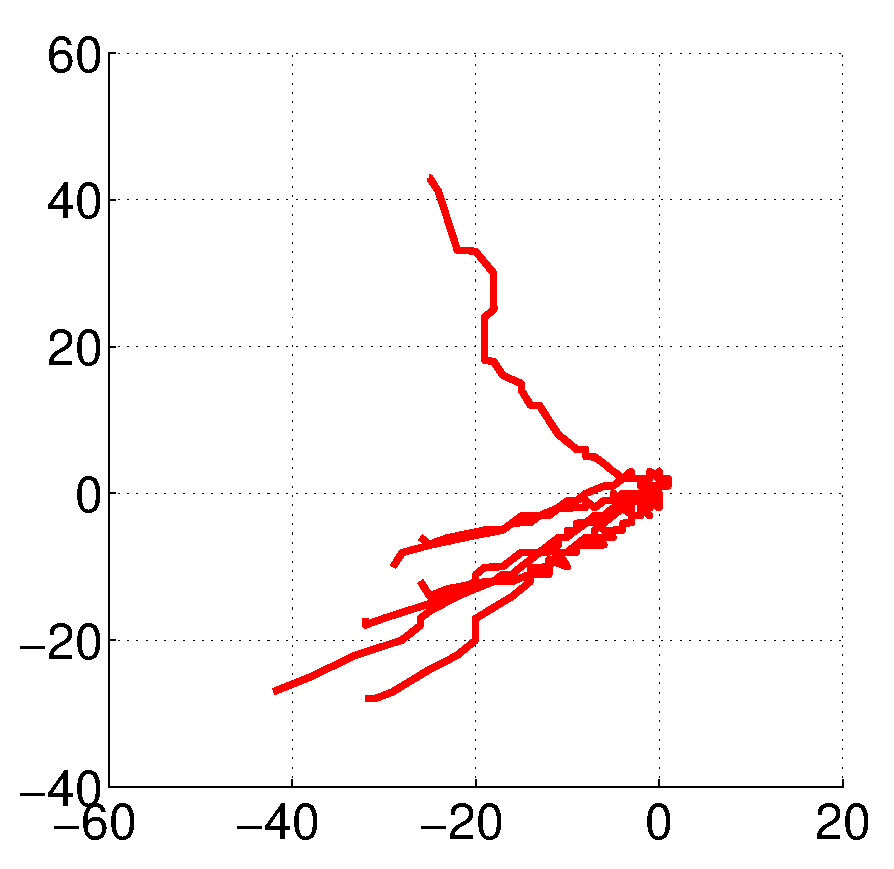
\includegraphics[width=30mm]{Figure/LeftEyeClosedLoop.eps}}  & \hspace{.1cm} &
	  \parbox{30mm}{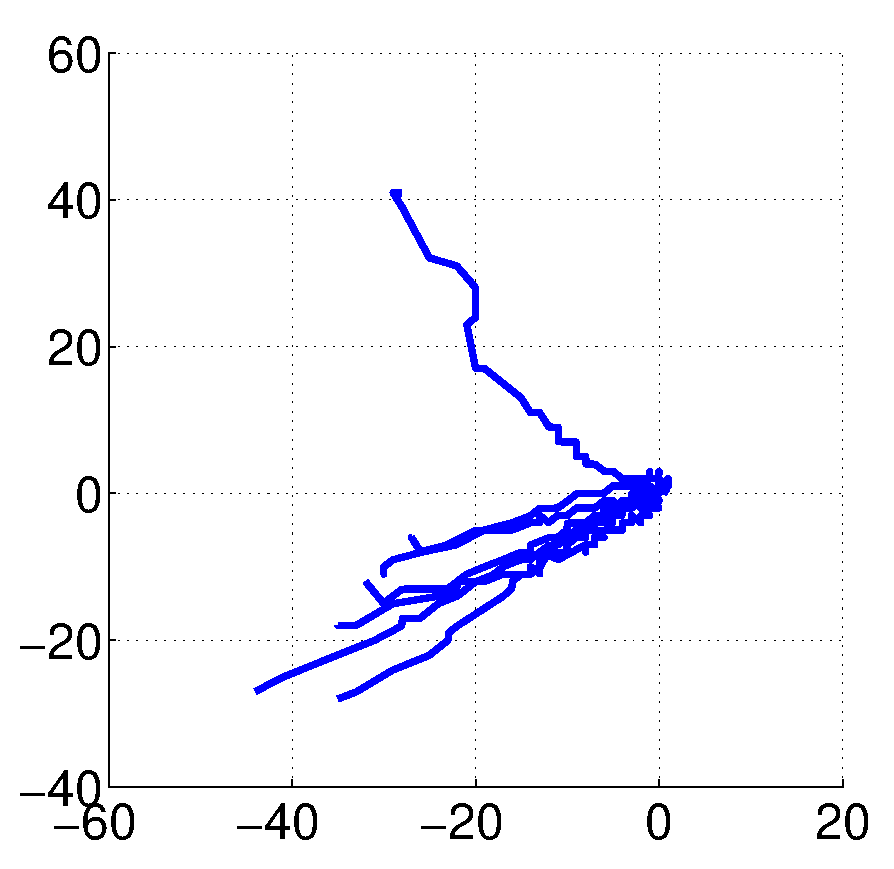
\includegraphics[width=30mm]{Figure/RightEyeClosedLoop.eps}}
	  \\
	  \parbox{30mm}{\centering Left eye } & \hspace{0.1cm} & \parbox{30mm}{\centering Right eye }
	  %	  \end{t\\
	  %	Top view & & Lateral view
  \end{tabular}
\end{center}
\caption{Traces of different closed loop control actions. Each trace correspond to a different Cartesian position of the target to be reached (which 
is always at the center of the image planes). All the traces end up in the image center thus indicating that the visual errors are completely eliminated by the closed loop controller.}\label{Fig:ImagePlaneClosedLoopErrors}
  \end{figure}

%\begin{figure}
%  % Requires \usepackage{graphicx}
%  \begin{center}
%	\begin{tabular}{ccc}
%	  \parbox{30mm}{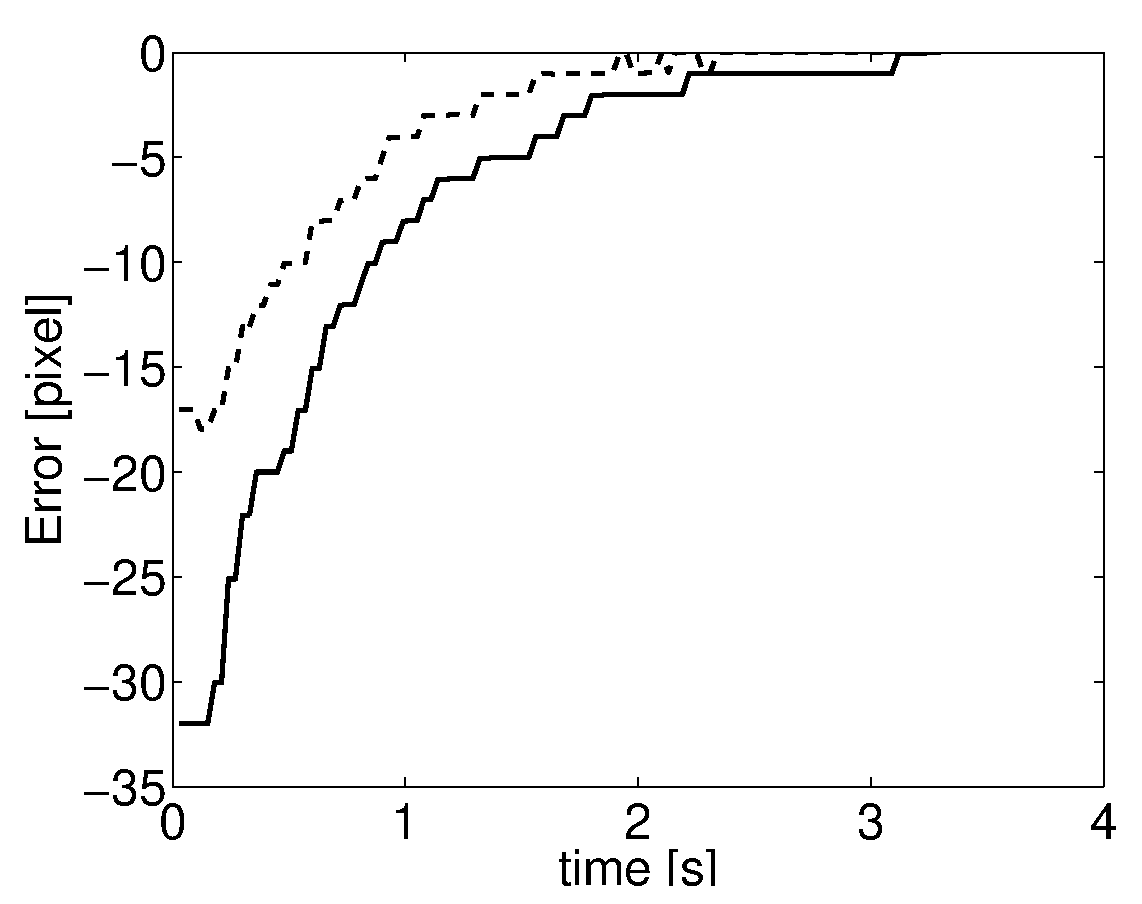
\includegraphics[width=30mm]{Figure/TimeReponseLeftClosedLoop.eps}}  & \hspace{.1cm} &
%	  \parbox{30mm}{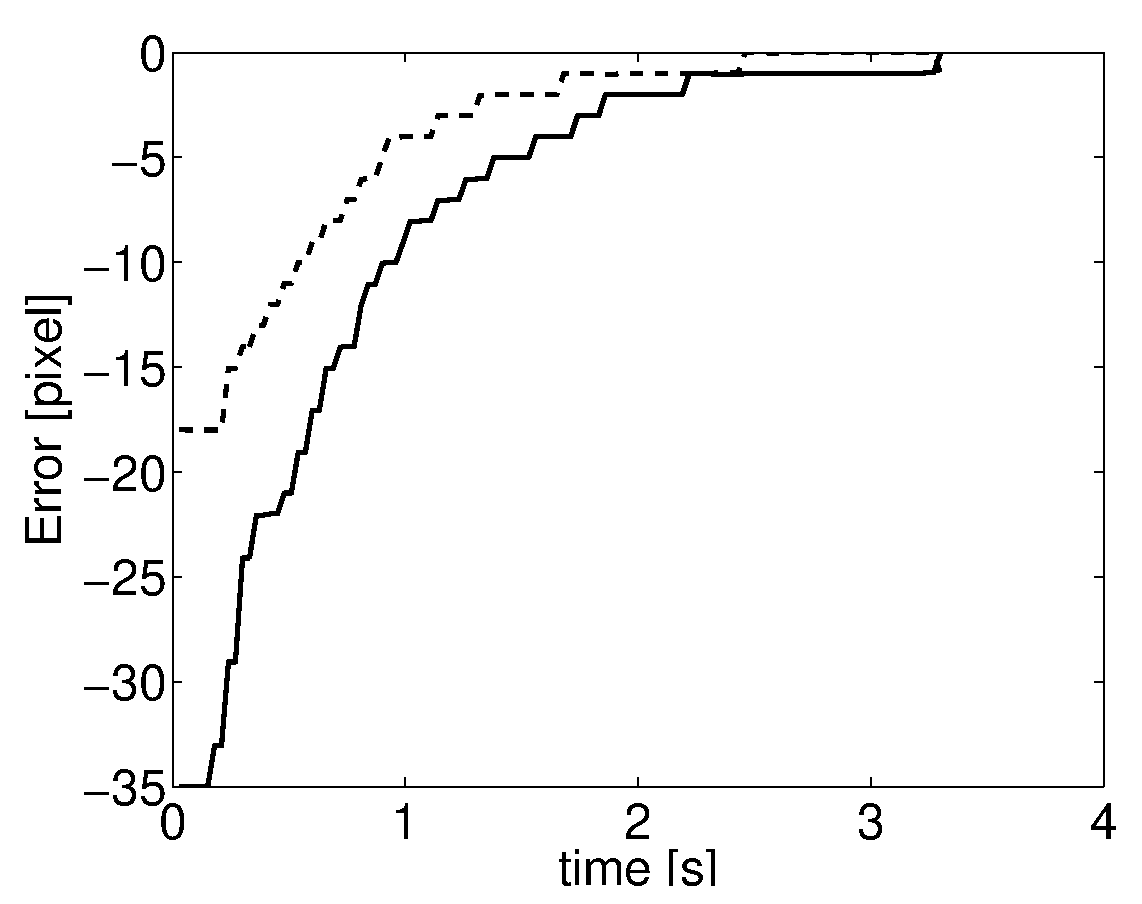
\includegraphics[width=30mm]{Figure/TimeReponseRightClosedLoop.eps}}
%	  \\
%	  \parbox{30mm}{\centering Left eye } & \hspace{0.1cm} & \parbox{30mm}{\centering Right eye }
%	  %	  \end{t\\
%	  %	Top view & & Lateral view
%  \end{tabular}
%\end{center}
%\caption{Time response of the closed loop controller. Solid lines: hand horizontal position in the left ($u_l$) and right ($u_r$). Dashed lines: vertical position, $v_l$ and $v_r$.}\label{Fig:TimeResponseClosedLoopErrors}
%  \end{figure}


\begin{figure}[th!]
  % Requires \usepackage{graphicx}
  \begin{center}
	\begin{tabular}{ccc}
	  \parbox{30mm}{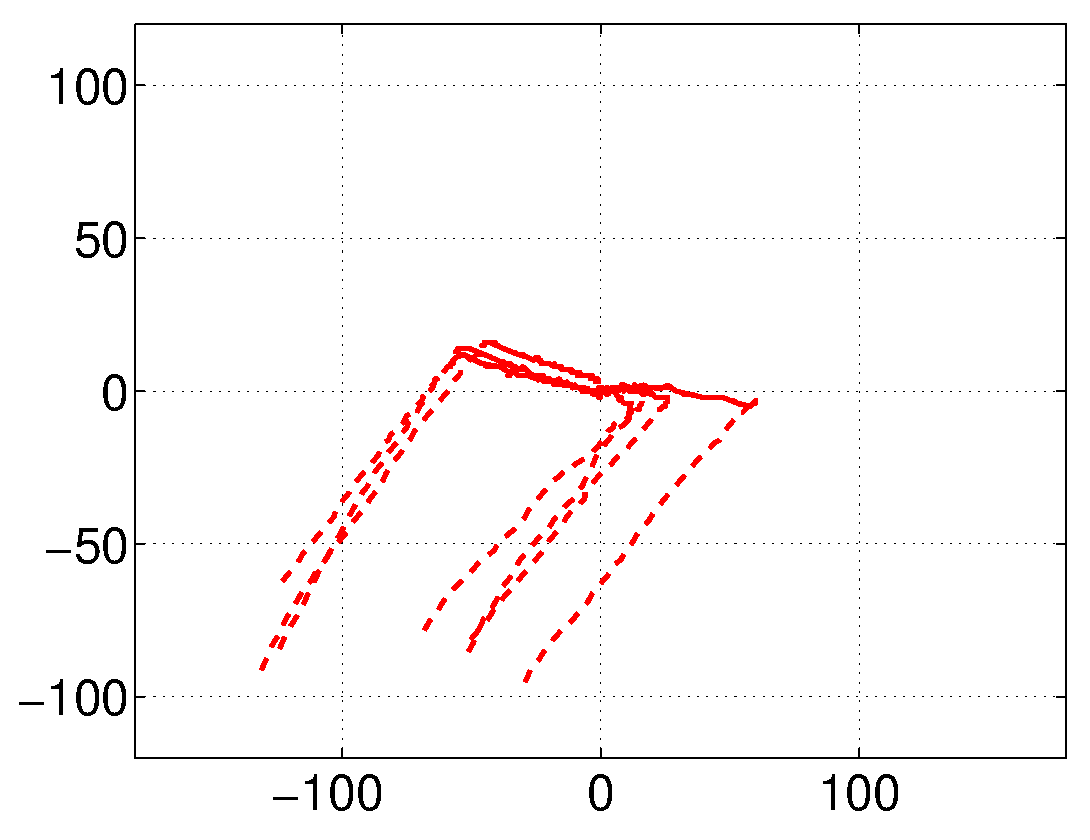
\includegraphics[width=30mm]{Figure/LeftEyeOpenClosedLoop.eps}}  & \hspace{.1cm} &
	  \parbox{30mm}{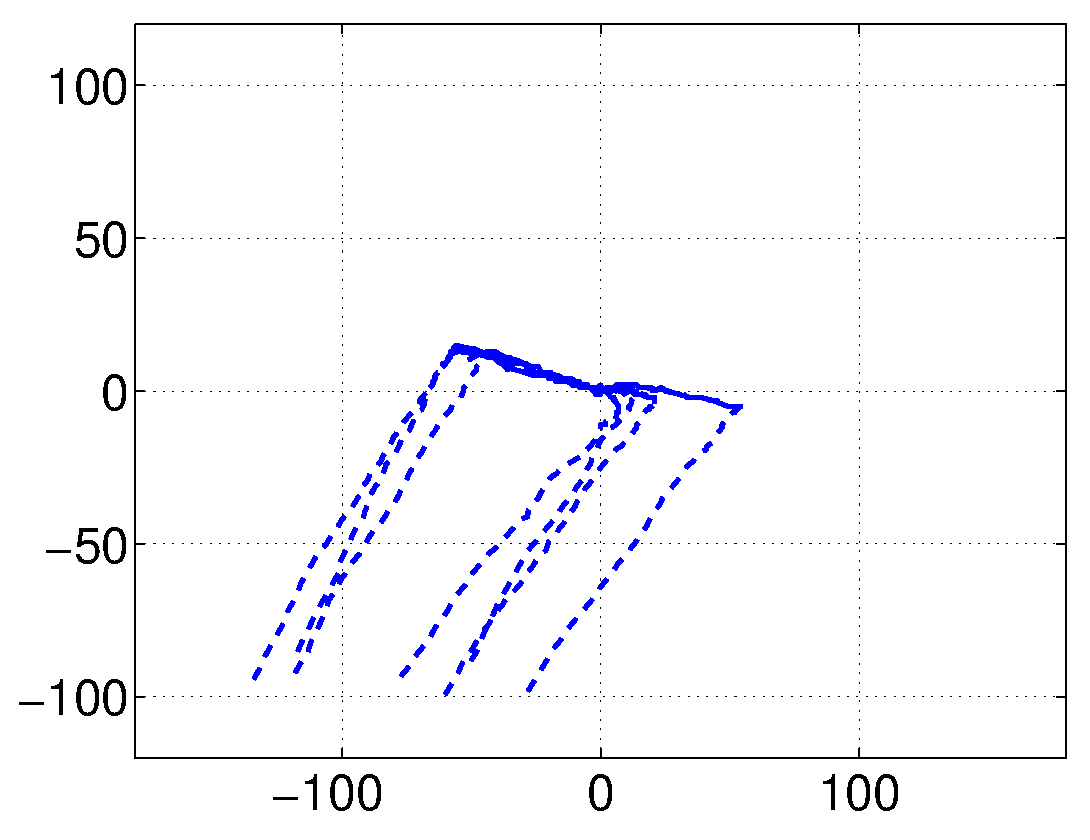
\includegraphics[width=30mm]{Figure/RightEyeOpenClosedLoop.eps}}
	  \\
	  \parbox{30mm}{\centering Left eye } & \hspace{.1cm} & \parbox{30mm}{\centering Right eye }
	  %	  \end{t\\
	  %	Top view & & Lateral view
  \end{tabular}
\end{center}
\caption{Movement of the hand on the image planes (320$\times$240)
during the execution of different reaching actions. 
Solid line: closed loop. Dashed trace: open loop. Clearly the open loop movement drives the hand to the target (the image centers) with a 
relatively small error. The closed loop phase reduces this error to zero.}\label{Fig:TimeResponseOpenClosedLoopErrors}
  \end{figure}
  
  \begin{figure}[th!]
  % Requires \usepackage{graphicx}
  \begin{center}
	\begin{tabular}{ccc}
	  \parbox{30mm}{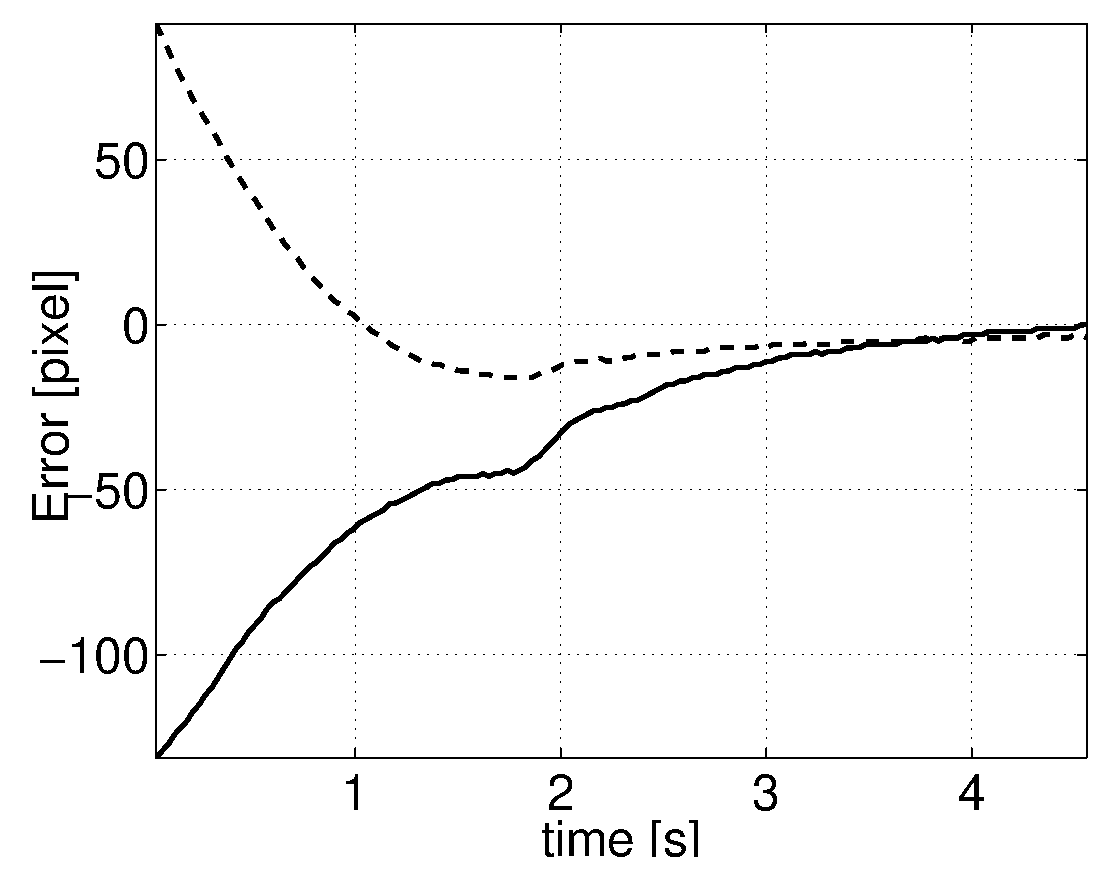
\includegraphics[width=30mm]{Figure/LeftEyeOpenClosedLoopTimeResponse.eps}}  & \hspace{.1cm} &
	  \parbox{30mm}{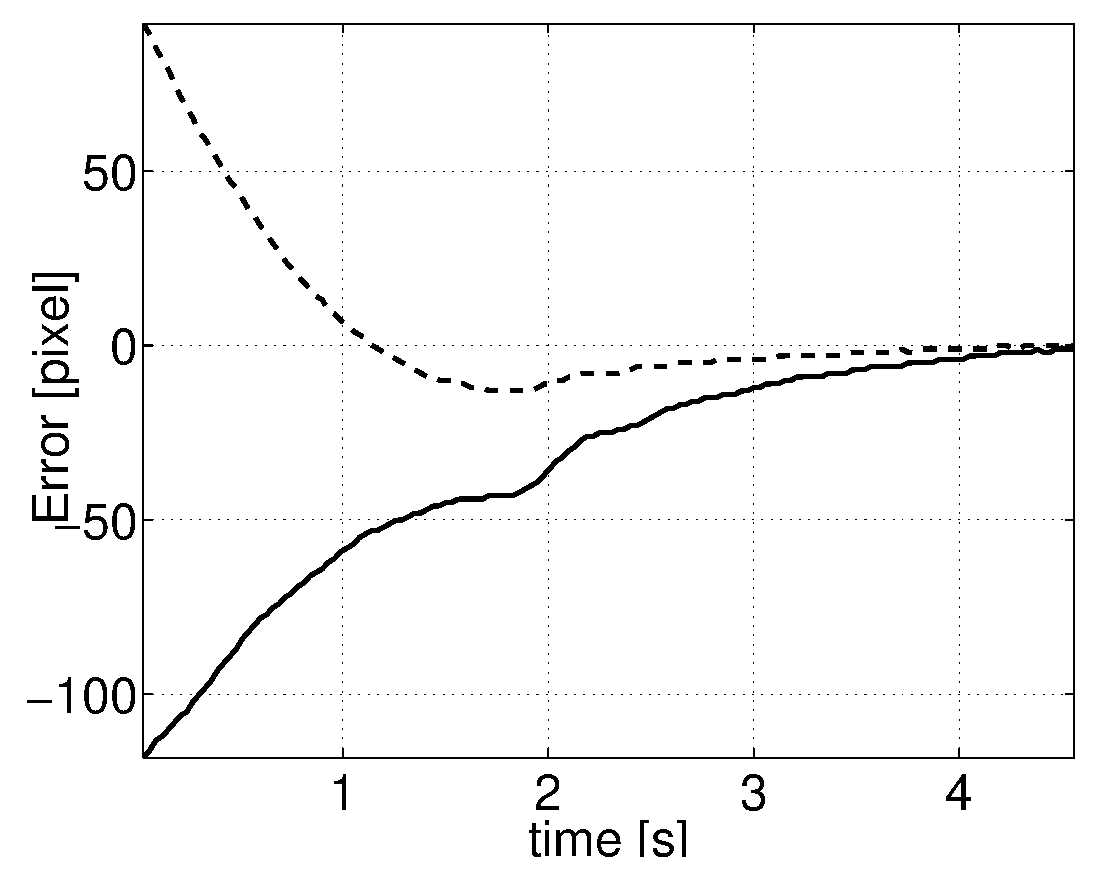
\includegraphics[width=30mm]{Figure/RightEyeOpenClosedLoopTimeResponse.eps}}
	  \\
	  \parbox{30mm}{\centering Left eye } & \hspace{.1cm} & \parbox{50mm}{\centering Right eye }
	  %	  \end{t\\
	  %	Top view & & Lateral view
  \end{tabular}
\end{center}
\caption{Time response of the closed loop and open loop strategy. Solid lines: $u_r$ and $u_l$. Dashed lines: $v_r$ and $v_l$. Remarkably, the open loop phase is faster but does not drive the hand exactly on the target. The closed loop is slower but more accurate.}\label{Fig:TimeResponseOpenClosedLoop}
\end{figure}


\subsection{Superimposed Open and Closed Loop}

Finally, we tested an alternative control strategy based on activating the closed loop 
phase immediately after the hand becomes visible on both image planes. This second strategy
is such that the open a closed loop strategies will be active at the same time for a 
certain amount of time. 
\newpage 
The structure is based on a classical control scheme, which can be represented as follows:

\begin{figure}[th!]
\begin{center}
\includegraphics[scale = 0.25]{Figure/OpenVSClosedLoop.eps}
\end{center}
\end{figure}

Practically, the feedforward control corresponds to the open loop part of the reaching movement.
It is activated exactly as described in Section \ref{sec:openReaching} and therefore it does not
require the hand to be visible in the image plane. The feedback control
instead corresponds to the closed loop part of the movement and can be activated when the hand
has been localized in both the image planes. Practically, the final solution can be described by the 
following scheme:

\begin{figure}[th!]
\begin{center}
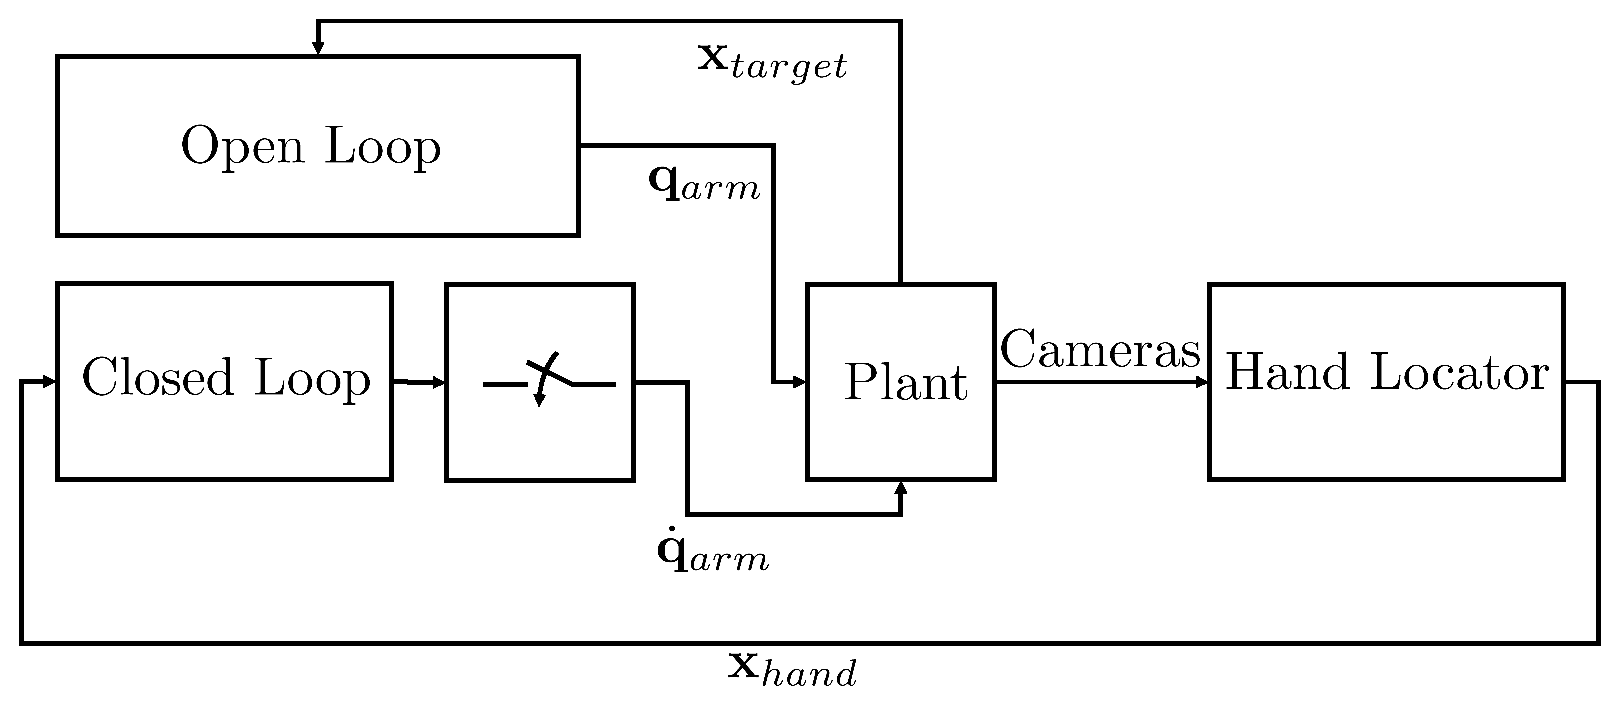
\includegraphics[scale = 0.25]{Figure/OpenVSClosedLoopSwitch.eps}
\end{center}
\end{figure}

Clearly, when both the open and closed loop controllers are active, the system receives position 
and velocity control simultaneously\footnote{A position command ${\mathbf q}_{arm,d}$ is 
always translated into a trajectory following command by moving 
the hand along a trajectory $\mathbf q_{arm}(t)$, $t \in [0, T]$ such that: $T$ is the execution time,
$\mathbf q_{arm}(0)$ is the arm position when the command is received, $\mathbf q_{arm}(T) = {\mathbf q}_{arm,d}$
is the desired final position, $\dot {\mathbf q}_{arm}(t) = 0$, $ \forall t > T$. If a velocity command $\dot {\mathbf q}_{arm,d}$ is received while executing a position
command $\mathbf q_{arm}(t)$, the original velocity command is transformed into a new one, nominally
$\dot {\mathbf q}_{arm} = \dot {\mathbf q}_{arm}(t) + \dot {\mathbf q}_{arm, d}$.}. 

A comparison between this control strategy and the one proposed in Section \ref{Eq:ClosedLoop}
is given in Figure \ref{Fig:TimeResponseOpenVSClosedLoopErrors} and \ref{Fig:TimeResponseOpenVSClosedLoop}. 
The second control strategy clearly outperforms the first one. As a matter of fact, the image plane movement (Figure \ref{Fig:TimeResponseOpenVSClosedLoopErrors})
is much more regular resulting in a unique linear movement instead of begin divided into two segments. Secondly, the
execution time is clearly reduced as it can be noted in Figure \ref{Fig:TimeResponseOpenVSClosedLoop}.


\begin{figure}
  % Requires \usepackage{graphicx}
  \begin{center}
	\begin{tabular}{ccc}
	  \parbox{30mm}{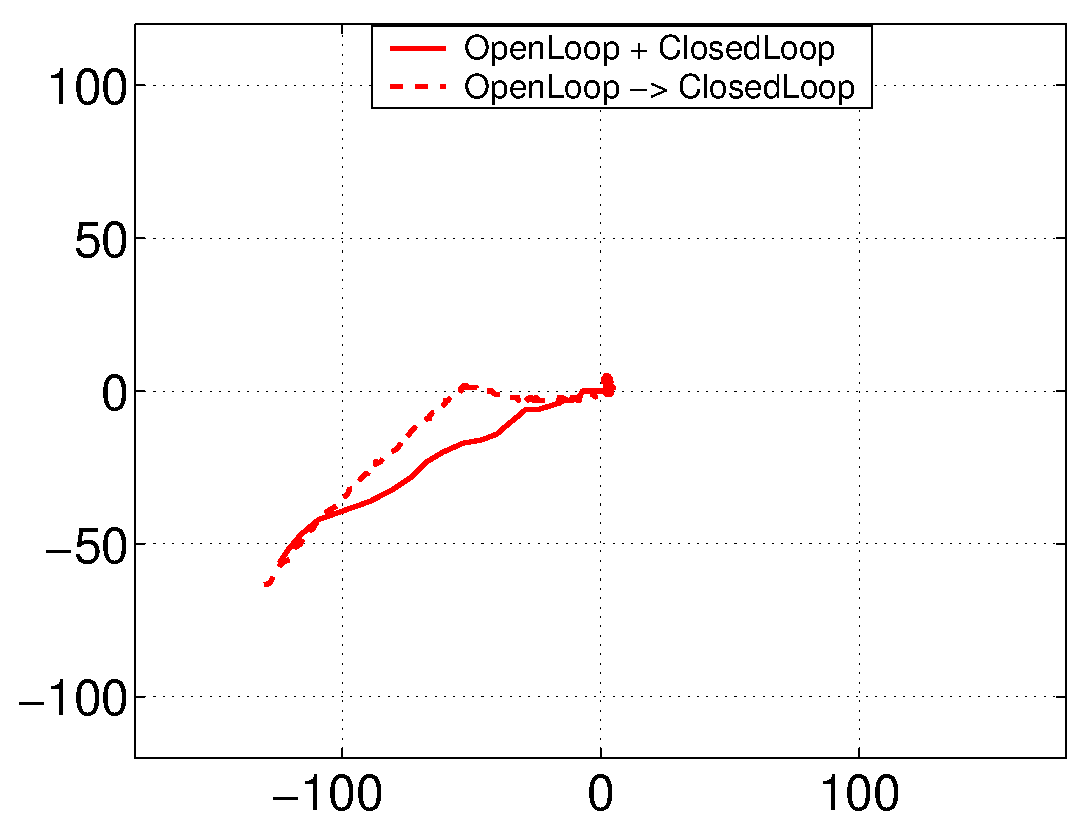
\includegraphics[width=30mm]{Figure/LeftEyeOpenVSClosedLoop.eps}}  & \hspace{.1cm} &
	  \parbox{30mm}{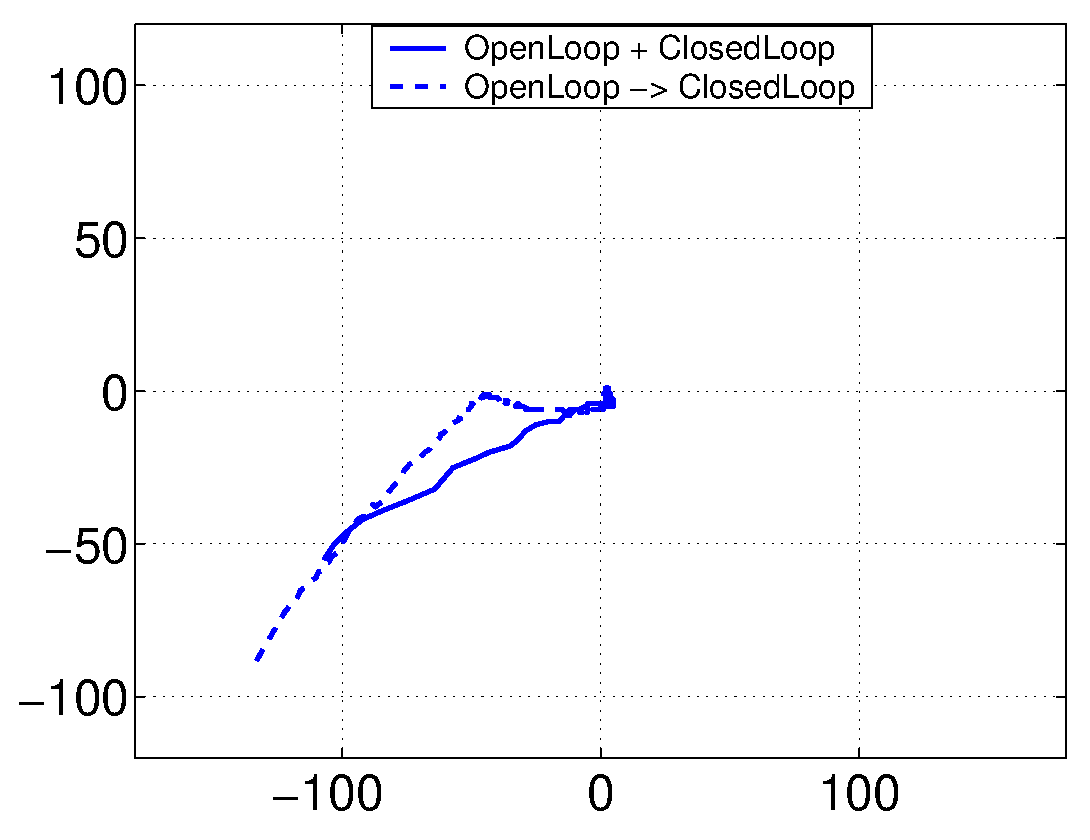
\includegraphics[width=30mm]{Figure/RightEyeOpenVSClosedLoop.eps}}
	  \\
	  \parbox{30mm}{\centering Left eye } & \hspace{.1cm} & \parbox{30mm}{\centering Right eye }
	  %	  \end{t\\
	  %	Top view & & Lateral view
  \end{tabular}
\end{center}
\caption{Movement of the hand on the image planes ($320 \times 240$)
during the execution of a single reaching movement. Dashed line: hand movement
during an open loop movement followed by a closed loop phase. Solid line: hand movement during 
the superposition of open and closed loop strategies.}\label{Fig:TimeResponseOpenVSClosedLoopErrors}
  \end{figure}
  
  \begin{figure}
  % Requires \usepackage{graphicx}
  \begin{center}
	  \parbox{40mm}{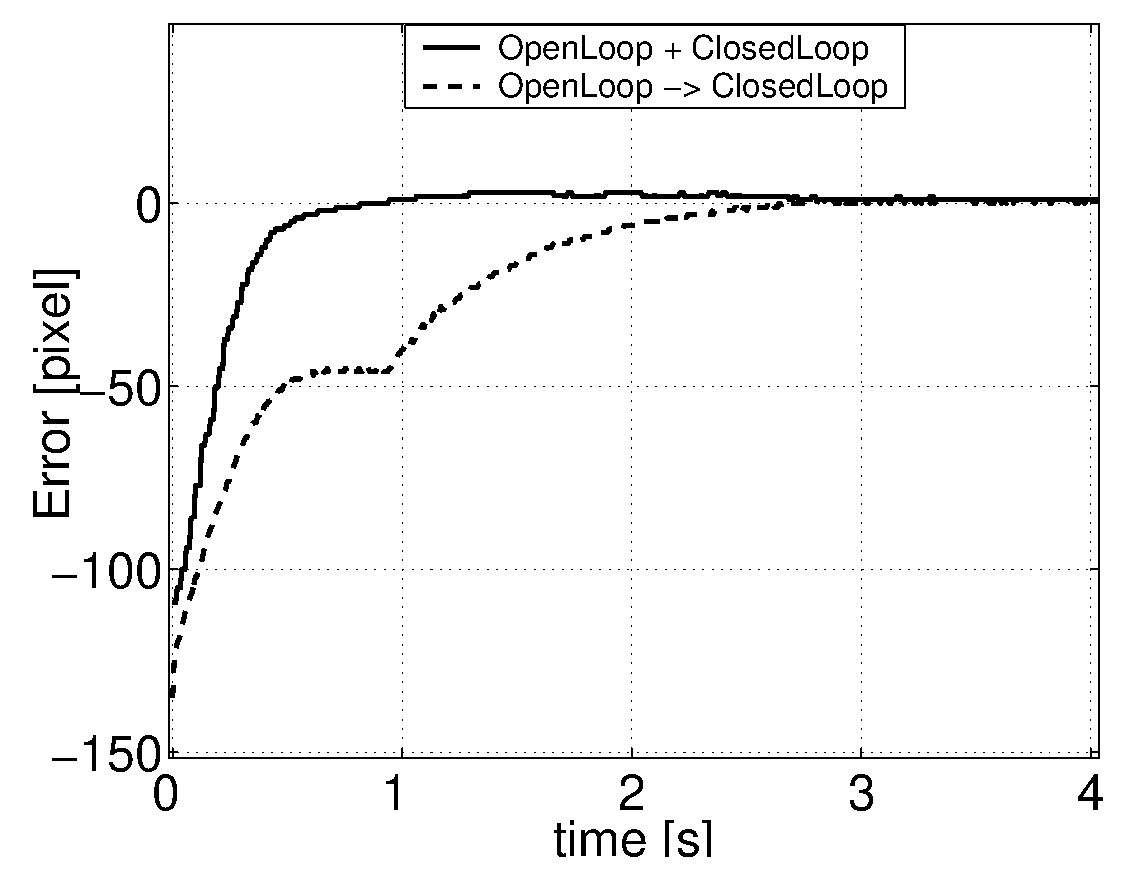
\includegraphics[width=40mm]{Figure/OpenVSClosedLoopTimeResponse1.eps}}
  \end{center}
\caption{Time response of the image plane position $u_l$. Dashed line: hand movement
during an open loop movement followed by a closed loop phase. Solid line: superposition of open and closed loop strategies.
 Remarkably, this second control architecture results in a faster response because when the hand becomes visible it is 
directly driven to the target without waiting for the open loop phase end.}\label{Fig:TimeResponseOpenVSClosedLoop}
  \end{figure}

\subsection{Null space movement}

In order to validate the quality of the Jacobian estimation, we tested the effects of a null space movement 
on the primary task (keeping $\uhand = 0$) as proposed in \cite{Mansard06jacobian}. A simple way to perform this testing is the following control strategy:
\begin{equation} \label{Eq:ClosedLoopStrategyRedundant}
\mathbf{\dot q}_{arm}=-k_1 \cdot \jacobian^\# \uhand + k_2 (I - \jacobian^\# \jacobian) \mathbf w, 
\end{equation}
where $I \in \mathbb R^{4 \times 4}$ is the identity matrix, $\mathbf w \neq 0$ is a 
randomly chosen vector in $\mathbb R^4$ and $k_1$, $k_2$ are positive constants. 
Ideally, the strategy (\ref{Eq:ClosedLoopStrategyRedundant}) should allow arm movements 
$\mathbf{q}_{arm} \neq 0$ while leaving the hand position $\uhand$ unperturbed. Practically we observed 
a minimal image plane movement (Figure \ref{Fig:RedundancyImagePlane})
as oppposed to a relatively large arm movement (Figure \ref{Fig:RedundancyArm}). These results 
further prove the quality of our Jacobian estimation.

\begin{figure}
  % Requires \usepackage{graphicx}
  \begin{center}
	\begin{tabular}{ccc}
	  \parbox{30mm}{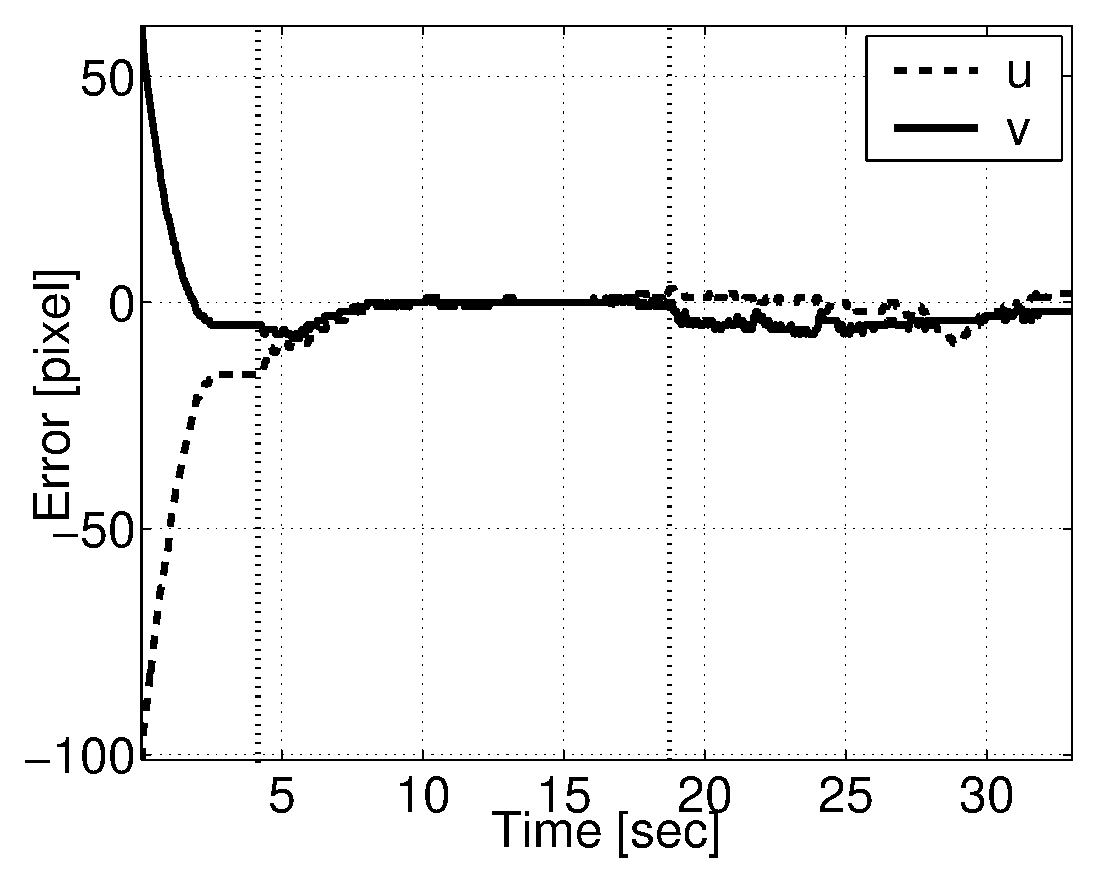
\includegraphics[width=30mm]{Figure/RedundancyLeft.eps}}  & \hspace{.1cm} &
	  \parbox{30mm}{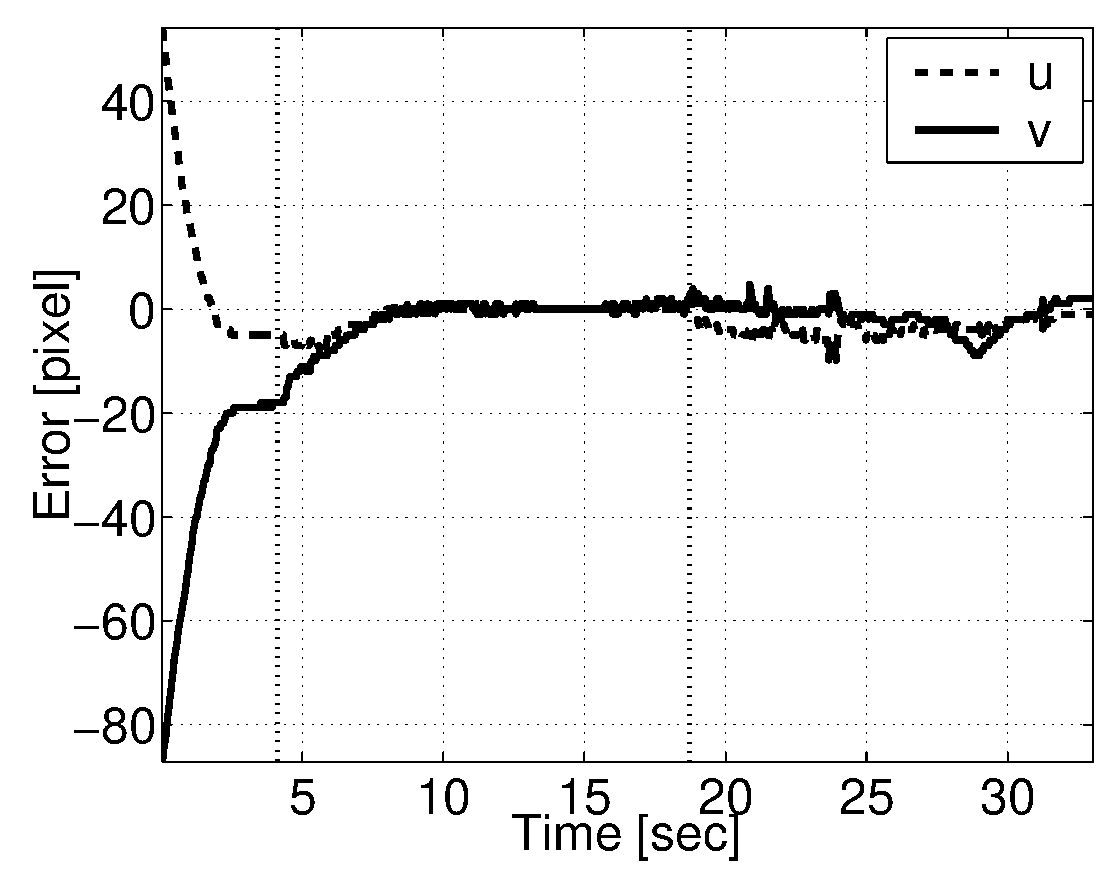
\includegraphics[width=30mm]{Figure/RedundancyRight.eps}}
	  \\
	  \parbox{30mm}{\centering Left eye } & \hspace{.1cm} & \parbox{30mm}{\centering Right eye }
	  %	  \end{t\\
	  %	Top view & & Lateral view
  \end{tabular}
\end{center}
\caption{Image plane movements during a three phase reaching. 
First the open loop, then the closed loop and finally a movement 
in the null space of the given task (keeping the hand in fixations). 
Each phase is delimited by a vertical dotted line.
}\label{Fig:RedundancyImagePlane}
  \end{figure}
  
  \begin{figure}
  % Requires \usepackage{graphicx}
  \begin{center}
	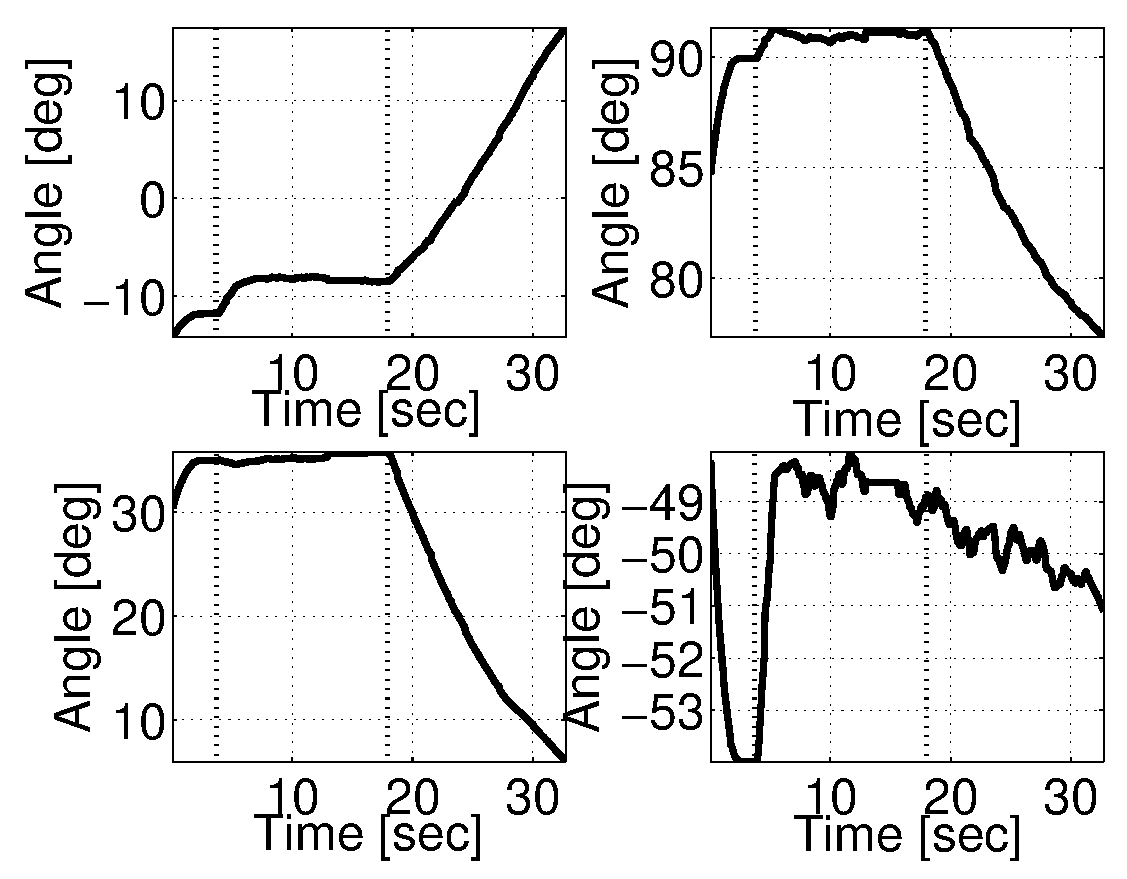
\includegraphics[width=60mm]{Figure/RedundancyArm.eps}
	\end{center}
\caption{Arm movement corresponding to the image plane movements shown in Figure \ref{Fig:RedundancyImagePlane}.
 Remarkably, the null space movement is characterized by large joint movements which are however not visible 
in the image plane due to the jacobian based compensation.} \label{Fig:RedundancyArm}
  \end{figure}
\section{Conclusions}
In this paper we have described the implementation of a reaching
behavior that integrates together an open loop and a closed 
loop controller. The open loop controller
allows the robot to perform faster movements and does not require visual 
feedback from the hand. When sight of the hand is available the closed
loop controller allows for precise positioning of the hand in the 
image plane. 

We describe an explorative strategy by which the robot autonomously 
acquires the forward motor map and the visual Jacobian transformations. 
Among the other things this strategy 
allows the estimation of the eye-to-hand visual Jacobian of the robot. 
The estimation of the Jacobian is a well studied task for which several 
solutions have been proposed \cite{Hosoda94versatile,Mansard06jacobian,
Lapreste04efficient}. None of these works, however, addresses the 
problem of the redundancy of both the head and the arm. In the experiments 
reported here the estimation of the Jacobian is performed with good 
accuracy for a subset of the arm workspace and for 
\emph{different head postures}. We believe
this is an important contribution with respect to the state of the art.

We do not rely on any prior information about the 
kinematic structure of the robot. The only simplification was that we used 
a color marker to visually localize the hand of the robot. Our assumption
is that the hand localization/identification is a separate problem
that needs to be solved before learning reaching. Previous work
by the same and other authors have suggested procedures by which 
the robot could autonomously learn to solve this task 
(\cite{Natale05,edsinger06what}). It will be interesting to see
how these approaches can be integrated with the work described 
in this paper.

\section*{Acknowledgements}
This research benefited from discussion with Giorgio Metta. 
The authors would like to thank Paul Fitzpatrick, Charles Kemp 
and Lijin Aryananda for providing some useful code. Funds for this 
project were provided by ABB, by the NASA Systems Mission Directorate,
Technical Development program under contract 012461-001, by 
DARPA DABT 63-00-C-10102, and by NTT under the NTT/MIT Collaboration 
Agreement. Lorenzo Natale was supported in part by the European Union 
grant RobotCub (IST-2004-004370).




%  Generate ``References'' here.
\bibliographystyle{sab}
\bibliography{natetorresj}

\end{document}
